%%%%%%%%%%%%%%%%%%%%%%%%%%%%%%
% 週報フォーマット
% 神経情報システム研究室
%%%%%%%%%%%%%%%%%%%%%%%%%%%%%%
\documentclass[dvipdfmx, A4j, twocolumn, 10.5pt]{jsarticle}
% \usepackage[doublespacing]{setspace} % ダブルスペースにしたいときはコメントを外す
\usepackage[margin=20truemm]{geometry} % 上下左右の余白は2cm
\usepackage{graphicx} % 図を挿入
\setlength{\columnsep}{2zw} % 列の間の空白

\usepackage{amsmath} % 数式?
% \usepackage{caption} % キャプションの追加
% \usepackage{biblatex} % 参考文献を扱うパッケージ
\usepackage{comment} % コメントを挿入する

% \addbibresource{references.bib} % リソースを取得


\begin{document}
%\thispagestyle{empty} % ページ番号はいらない

%%% タイトルなど
\twocolumn[%

\centering % 中央寄せ
{\fontsize{18pt}{18pt}\selectfont 週報}\\ % 和文題目
{\fontsize{12pt}{12pt}\selectfont 平岡立成}
\vskip\baselineskip % 一行空け
] 

%%% 本文
\section{今週やったこと}
\begin{itemize}
 \item 『神経回路シミュレーション』山崎匡 読み進め

\end{itemize}
\section{『神経回路シミュレーション』要約}

\section*{第1章 計算神経科学入門}
\subsection*{1.1 計算神経科学とは何か}
神経科学とは,医学,生物学,化学,心理学,情報科学等の集合体で,その中でも理論神経科学は,特に理論的な研究を主とする神経科学であり,数式等への抽象化をすることで脳のモデルを開発する.計算科学のアプローチをとるものをとくに計算神経科学と呼ぶが,理論神経科学と計算神経科学に明確な区別はない.とくに数値シミュレーションに特化した神経科学を「シミュレーション神経科学」と呼び,本書ではこれを扱う.

\subsection*{1.2 神経回路シミュレーション}
神経回路シミュレーションとは,脳の神経回路の挙動を計算機上で数値的にシミュレーションするもののことをいう.

\subsection*{1.3 ニューロンのモデル}
ニューロン(神経細胞)は,樹状突起,細胞体,軸索からなり,パラメータとして膜電位\footnote{細胞外を基準とした細胞内の電位}を持つ.膜電位のダイナミクスは次のように記述できる.

\begin{align*}
\frac{dV}{dt} = -\bar{g}_{\text{leak}} \left( V(t) - E_{\text{leak}} \right) + I_{\text{ext}}(t)
\end{align*}

これだけでは膜電位が上下するのみでスパイクは発射されない.膜電位は外部からの入力により値が変化し,ある閾値を超えるとスパイク\footnote{短い電気パルス.}を発射する.具体的には,スパイクは,Na\textsuperscript{+}イオンやK\textsuperscript{+}イオンが軸索の表面にあるチャネル\footnote{表面にあるイオンの通り道.刺激に応じて開閉をする.これを電位依存性という.}を通過することで生じる電流により生成する.それぞれの電流は次のように記述できる.

\begin{align*}
I_{\text{Na}}(t) &= -g_{\text{Na}}(V,t)(V(t) - E_{\text{Na}}) \\
I_{\text{K}}(t) &= -g_{\text{K}}(V,t)(V(t) - E_{\text{K}})
\end{align*}

$g_{\text{Na}}(V,t)$,$g_{\text{K}}(V,t)$は,Na\textsuperscript{+}チャネルとK\textsuperscript{+}チャネルのコンダクタンス\footnote{抵抗Rの逆数.電流の流れやすさを示す.}であり,時間と膜電位の関数となる.$E_{\text{Na}}$,$E_{\text{K}}$,は各イオンチャネルの反転電位である.

\begin{figure}[h]
 \centering
 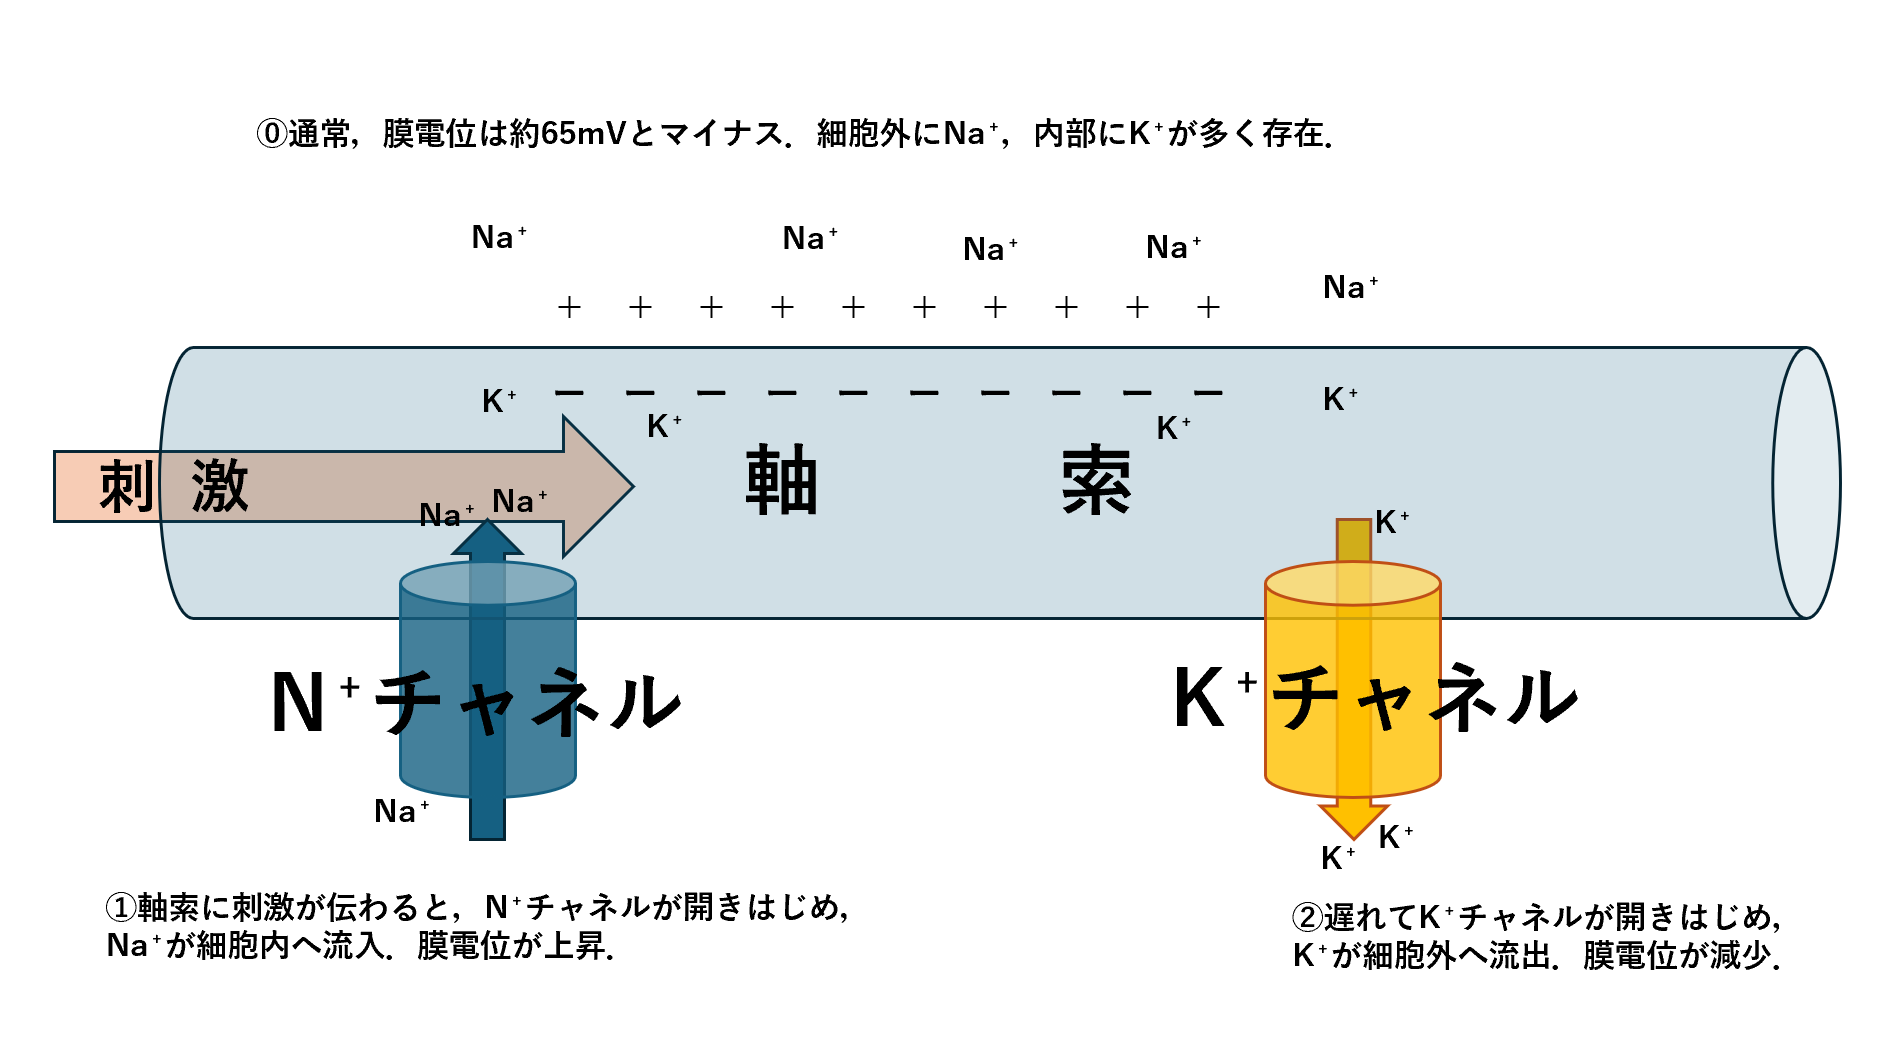
\includegraphics[width=0.45\textwidth]{spike.png}
 \caption{スパイク発生の流れ} 
\end{figure}


\begin{figure}[h]
 \centering
 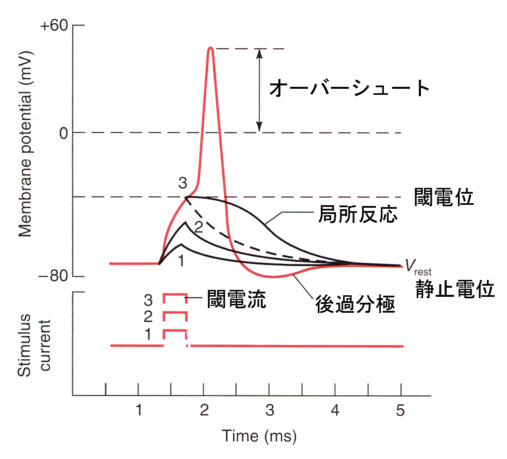
\includegraphics[width=0.45\textwidth]{actpot.jpg}
 \caption{静止電位と活動電位(スパイク) \cite{lite1}} 
\end{figure}

コンダクタンスの変化により,膜電位の値が急速に上下し,スパイクが生成される.コンダクタンスの式は動物やニューロンの種類により様々であり,世界初のコンダクタンスの式がヤリイカのニューロンを対象としたHodgkin-Huxley方程式である.

\subsection*{1.4 シナプスのモデル}
スパイクが末端のシナプスへ到達すると,シナプスから神経伝達物質が放出される.放出される神経伝達物質は,ニューロンの種類により異なる.
\begin{itemize}
 \item 興奮性ニューロン(シナプス)... グルタミン酸
 \item 抑制性ニューロン(シナプス)...GABA(γアミノ酪酸)
\end{itemize}

% \printbibliography

これが他のニューロンの樹状突起へ到達すると電流が流れる\footnote{これをシナプス電流という.}.興奮性シナプスからは,脱分極させる電流\footnote{興奮性後シナプス電流,EPSC},抑制性シナプスからは過分極させる電流\footnote{抑制性後シナプス電流,IPSC}がそれぞれ発生する.

\begin{figure}[h]
 \centering
 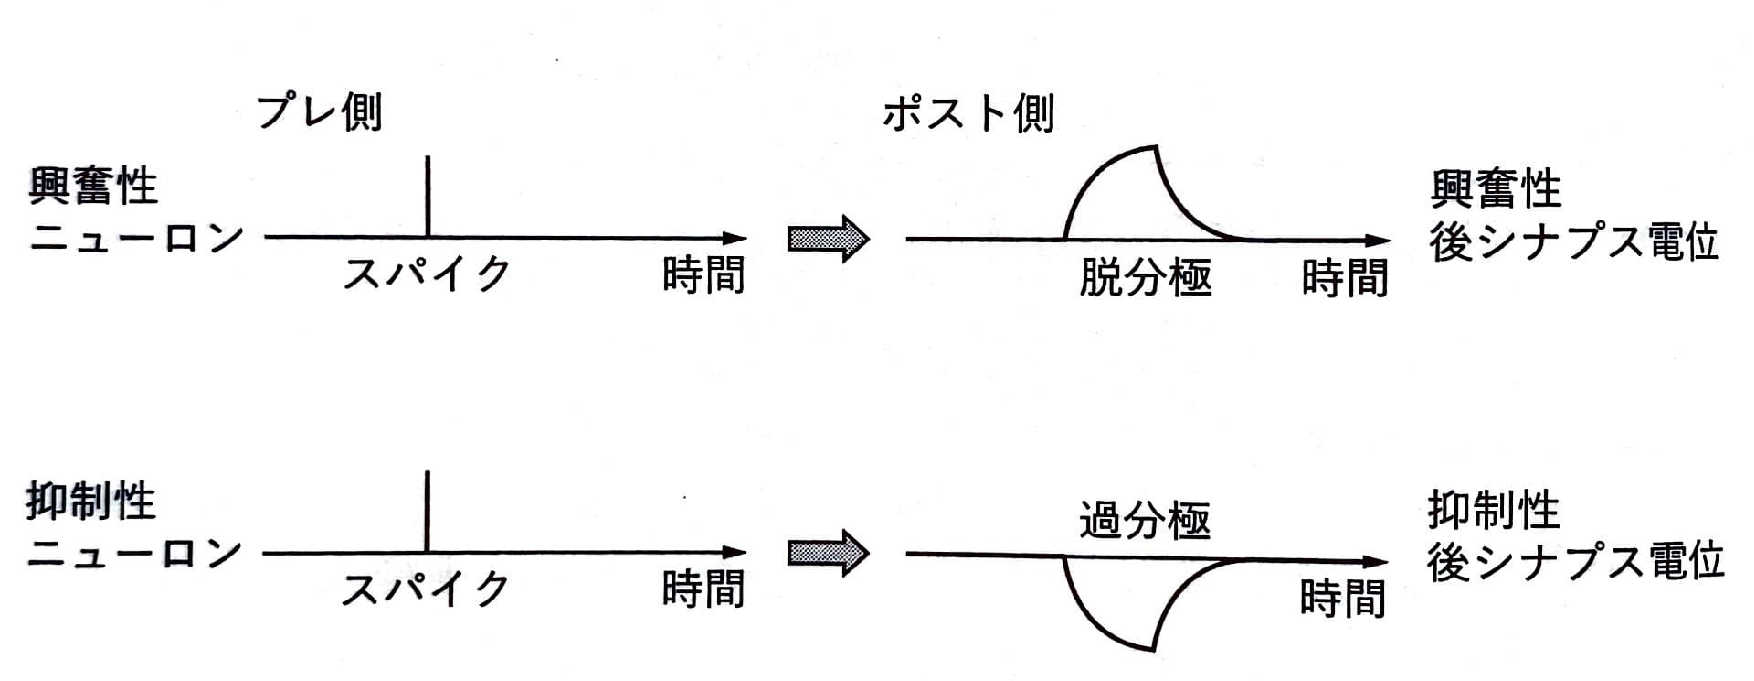
\includegraphics[width=0.45\textwidth]{isyn.pdf}
 \caption{各シナプス電流による,シナプス電位発生の様子}
\end{figure}

シナプス電流$I_{\text{syn}}$も,シナプスコンダクタンス$g_{\text{syn}}(t)$を用いて次のようにかける.

\begin{align*}
 I_{\text{syn}}(t) = -g_{\text{syn}}(t) \left( V(t) - E_{\text{syn}} \right)
\end{align*}


$E_{\text{syn}}$はシナプスの反転電位\footnote{興奮性シナプスでは0mV,抑制性シナプスでは-65~80mV.}を示す.


\section*{第2章 常微分方程式の数値解法}

\subsection*{2.1 常微分方程式の初期値問題}
$x(t)$を時間tに関する変数とし,その時間変化が$f(x, t)$で与えられるとする.

\begin{equation}
  \frac{dx}{dt} = f(x, t)
\end{equation}
\begin{equation}
  x(0) = x_0
\end{equation}


2つ目の式はxの時刻t=0における値で,初期条件という.2つの式は,ただ1つの自由変数tを持つ.このような微分方程式を常微分方程式と呼ぶ.先程のニューロンの膜電位の式もこの形をとる.これを数値的に解く方法として,オイラー法,ホイン法,ルンゲクッタ法\footnote{こういった方法のことを数値解法という}などがある.

\subsection*{2.2 オイラー法}
常微分方程式を数値的に解く最も簡単な方法がオイラー法(Euler法)である.数学的に微分の定義は

\begin{equation}
  \frac{dx}{dt} = \lim_{\Delta t \to 0} \frac{x(t + \Delta t) - x(t)}{\Delta t}
\end{equation}

であるが,コンピュータ上で無限に小さい値を扱うことはできないので,代わりに十分小さい値$\Delta t$を用いて

\begin{equation}
  \frac{dx}{dt} \approx \frac{x(t + \Delta t) - x(t)}{\Delta t}
\end{equation}


と近似する.この式を変形すると,

\begin{equation}
 x(t+\Delta t)=x(t)+\Delta t f(x, t)
\end{equation}


が得られる.オイラー法は簡単な手法だが精度の悪い方法である.$x(t+\Delta t)$を$t$周りでテイラー展開すると,

$$
\begin{aligned}
x(t+\Delta t) & =x(t)+\frac{1}{1!} f(x, t) \Delta t+\frac{1}{2!} f^{\prime}(x, t) \Delta t^2+\cdots \\
& =x(t)+\frac{1}{1!} f(x, t) \Delta t+O\left(\Delta t^2\right)
\end{aligned}
$$

となる.2式を比較すると,オイラー法は,1次の項までが一致しており,2次以降の後を無視した計算法であることがわかる.オイラー法の誤差はO記法により,O($\Delta t$)と記述することができる.これは$\Delta t$の値を1/100倍すると,誤差も1/100倍となることを意味する.

\subsection*{2.3 ホイン法,ルンゲクッタ法}
その他の方法の詳細な説明は割愛するが,ホイン法の場合,その誤差はO($\Delta t^2$)となる.これは,$\Delta t$が1/100倍されれば,その誤差は1/10000倍にまで減少できることを意味する.
さらに,(4次の)ルンゲクッタ法においてはその誤差はO($\Delta t^3$)まで減少し,さらに精度が高くなることがわかる.

\section*{次週の予定}

\begin{itemize}
 \item hodgkin-huxleyモデルと積分発火型モデルの理解

\end{itemize}


\begin{thebibliography}{99}
\bibitem{lite1} 和田勝 ``筋肉による筋収縮の司令'' 生命科学C, 2001, https://www.tmd.ac.jp/artsci/biol/textlife/neuron.html.
% \bibitem{lite2} R. Hosaka, T. Kimura, and T. Matsuura, ``title,'' journal name, pp.10-20, 2021.
\end{thebibliography}
\end{document}
